%\documentclass[journal]{IEEEtran}
\documentclass[oneside]{article}

\usepackage{graphicx}\usepackage{url}  % code reduction referencing pictures 
\usepackage{amsmath}  % Complies math
\usepackage{fancyhdr}  % Headers and footers
\usepackage{hyperref}  % Enable Hyperlinks
\usepackage{algpseudocode}  % for writing pseude code
\usepackage{geometry}  

% change page margins
\geometry{  
a4paper,
left=30mm,
right=30mm,
top=30mm,
bottom=20mm
}


\begin{document}

\begin{titlepage}
   \begin{center}
        \vfill
        \textit{Report for Final Project}\\
        \textit{In Class Optimization}\\
        \vspace{0.5cm}
        Advisors:\\
        \textit{Assistant Professor Imre Fekete}\\
        \textit{Sebastian Kusch}
        \vfill\noindent\hrulefill \\
        \vspace*{1cm}
        \textbf{\huge ADAM}\\
        \vspace{0.5cm}
        
         Adaptive Movement Estimation Algorithm
        
        \noindent\hrulefill \\

       
            
       \vspace{1.5cm}

       \textbf{Olle Rehnfeldt \& Jakob Hutter}

       \vfill
            
       
            
       \vspace{2cm}
       BSc Data Science and Society\\
       Central European University\\
       Quellenstraße 51, 1100 Vienna, Austria\\
       31st of March 2024\\
       \vspace{1.5cm}
       
\includegraphics[width=0.4\textwidth]{figures/CEU_Logo_RGB_DualColor.png}
       
            
   \end{center}
\end{titlepage}






% FOOTER AND HEADER SETTINGS
\pagestyle{fancy}
%\headheight = 25pt
%\fancyhf{}
%\fancyfoot[C]{\thepage}
%\fancyhead[C]{Adaptive Movement Estimation Algorithm \\ \nouppercase{\leftmark\hfill\rightmark}}

\newpage

% TABLE of Content
\tableofcontents 
\vspace{1.5cm}


%%%%%%%%%%%%%%%TODOS
% instead of \\ do the \par
% never use png, save it as PDF
% steps in algorithm make bolt

% FUSE some paragraphs, be more precise and summarize
    % DONE -- FUSE ONE AND TWO
    % DONE -- FUSE THREE AND FOUR
    % FUSE FIVE AND SIx
%label graphs and equations
    % UTILIZE BEGIN EQUATION \label{eq:name}  \ref{eq:name}
        % theta add t
    % do the same for figures
%%%%%%%%%%%%%%

\newpage
% START PAPER here
\section{Introduction}
This paper delves into the intricacies of optimization algorithms pivotal to machine learning, with a spotlight on ADAM, an algorithm that combines the features of RMSprop and Momentum into the stochastic gradient descent (SGD) framework. Setting the stage with an overview of Gradient Descent (GD) and its stochastic variant, SGD, we pave the way for a nuanced discussion on ADAM. ADAM stands out for its dynamic learning rate adjustment and incorporation of momentum, strategies that enhance the efficiency of navigating the complex optimization terrain of large datasets and neural network architectures. Through this introductory exploration, we aim to showcase how ADAM's innovative approach to parameter updates not only accelerates convergence but also offers a significant advantage in flexibility and robustness over traditional methods, marking a pivotal evolution in the optimization strategies for machine learning applications. After the introduction and the explanation of ADAM's operating principles, we analyze ADAM's performance compared to other optimization algorithms through some examples 
\subsection{Gradient Descent}
Gradient Descent is an optimization algorithm utilized for minimizing the loss function. In the context of a Neural Network application, GD updates the model's parameters (for example, weights) by moving them in the direction opposite to the gradient of the loss function concerning those parameters, to minimize the loss.\par
A commonly employed metaphor is that of a hiker in the mountains, which represents the landscape of the loss function. The hiker's goal is to reach the lowest valley within the mountain range, where the loss is minimal; at the mountain peaks, the loss is maximal, and in the valleys, it is lowest. The challenge for the hiker arises in bad weather conditions, where visibility of both the peak and the valley is obstructed. In this scenario, Gradient Descent aids the hiker by calculating the direction from their current position where the mountain has the steepest downward gradient. By repeatedly following the direction of the gradient, the hiker will eventually reach a valley, which corresponds to a local minimum of the loss function.\par

\subsubsection{Application in Neural Networks}
Introducing the notion of parameters:
\begin{itemize}
    \item \( \theta \):\par The parameters of the model.
    \item \( \alpha \):\par  The learning rate, a small positive scalar determining the size of the steps. It's crucial for convergence: too small, and the optimization is slow; too large, and you may overshoot the minimum.
    \item \( \nabla_\theta J(\theta) \):\par  The gradient of the loss function \( J \) with respect to the parameters \( \theta \). This gradient points in the direction of the steepest increase of \( J \); hence, moving against it leads to the steepest decrease.
\end{itemize}
This is the formula of gradient descent to update the gradient at the current point:
\begin{equation}
    \theta_t = \theta_{t-1} - \alpha \nabla_\theta J(\theta)
    \label{eq:theta}
\end{equation}
In Eq.\ref{eq:theta}
In the context of neural networks, GD therefore adjusts the weights and biases in a way that minimizes the difference between the predicted output and the actual output (the loss). Here's a simplified view of the process:
\begin{enumerate}
    \item  \textbf{Initialization}:\par
    Start with random weights and biases for your neural network.
    \item  \textbf{Forward Pass}: \par
    Input data through the network and compute the output.
    \item  \textbf{Compute Loss}: \par
    Use a loss function to calculate the error between the predicted output and the actual output.
    \item  \textbf{Backward Pass (Backpropagation)}:\par
    Calculate the gradient of the loss function concerning each weight and bias in the network. This is where calculus comes into play, as you're essentially finding out how to tweak the weights and biases to reduce the loss.
    \item  \textbf{Update Parameters}:\par
    Adjust the weights and biases in the opposite direction of their gradients to minimize the loss, using the learning rate to scale the size of the update.
    \item  \textbf{Repeat}: \par
    Repeat steps 2-5 for many iterations (epochs) until the loss converges to a minimum value, indicating that the model's predictions are as accurate as possible with the given architecture and data.
\end{enumerate}\par
By iteratively applying Gradient Descent, neural networks can be trained to execute predictions or classifications with notable accuracy. This methodology is fundamental to the training phase of machine learning and deep learning models. However, to address this limitation, we will explore Stochastic Gradient Descent as an enhancement in the subsequent section.
\subsection{Stochastic Gradient Descent}
Stochastic Gradient Descent is a variation of the basic GD algorithm that introduces randomness in the optimization process to achieve faster convergence and potentially escape local minima.\par
In the standard GD, you calculate the gradient of the loss function using the entire dataset to make a single update to the parameters. This approach, while effective, can be slow and computationally expensive for large datasets, as you need to process all data points before making even a small step in parameter space.\par
SGD modifies this process by updating the model's parameters using only a single data point ( or a small batch of data points) at a time. Here's how it works in steps:
\begin{enumerate}
    \item \textbf{Randomly Shuffle the Dataset}\par
    Initially, the data is shuffled to ensure that the order does not affect the optimization.
    \item \textbf{Select One Data Point (Stochastic GD)} or a Small Batch (Mini-batch SGD)\par
    Instead of using the entire dataset to compute the gradient of the loss function, select a single data point or a small subset of the data.
    \item \textbf{Compute the Gradient}\par
    Calculate the gradient of the loss function concerning the parameters, but only for the selected data point or batch. This gradient is an estimate of the gradient over the entire dataset.
    \item \textbf{Update the Parameters}\par
    Use this estimated gradient to update the model's parameters, similar to the basic GD formula:
    \begin{equation}
        \theta = \theta - \alpha \nabla_\theta J(\theta; x^{(i)}, y^{(i)})
        \label{eq:SGD}
    \end{equation}
    In Eq.\ref{eq:SGD}, \(x^{(i)}\) and \(y^{(i)}\) represent the input features and the target output of the selected data point(s), respectively.
    \item \textbf{Repeat} \par
    Continue this process, iterating through the dataset in small increments (single data points or batches), updating the model's parameters each time till $\theta$ converges.
\end{enumerate}

Switching from GD to SGD offers several benefits, including faster convergence, as it updates parameters more frequently, making it quicker to reach the minimum of the loss function, especially beneficial for large datasets. It also reduces memory usage by utilizing only a fraction of the data at each step, enabling training on large datasets that cannot fit entirely in memory. Additionally, the inherent noise and randomness in the selection of data points or batches with SGD can assist the optimization process in escaping local minima, potentially finding better solutions that standard GD might miss. SGD's flexibility to adjust learning rates and batch sizes allows for a balance between speed of convergence, computational resource management, and training stability, making SGD particularly well-suited for large-scale machine-learning challenges.


\subsection{ADAM}
ADAM is an advanced optimization algorithm designed to improve the training efficiency of machine learning models by merging the principles of RMSprop (Root Mean Square Propagation) and Momentum with SGD. This synthesis allows for dynamic adjustment of learning rates for each parameter based on estimates of gradients' first and second moments, leading to quicker and more effective convergence than traditional SGD, especially beneficial for processing large datasets and managing complex neural network architectures. By building upon the foundation laid by both gradient GD and SGD—where GD methodically updates model parameters across the entire dataset but at a slower, more resource-intensive pace, and SGD introduces a beneficial level of noise through updates based on single samples or small batches—ADAM optimizes this process. It not only embraces the stochastic nature of SGD but enhances it by incorporating adaptive learning rates and momentum, tracking exponentially decaying averages of past gradients and squared gradients to fine-tune each parameter's learning rate, making it highly effective for scenarios with sparse gradients or varied parameter sensitivities.

In the realm of deep learning, ADAM stands out for several reasons: it adjusts learning rates per parameter, enabling efficient handling of sparse gradients and varied parameter sensitivities—crucial for complex model architectures with numerous parameters. Similar to SGD, it is adept at working with mini-batches, facilitating efficient training on large datasets and accelerating convergence beyond the capabilities of SGD and traditional GD. Furthermore, ADAM's design reduces sensitivity to hyperparameter selection, notably the initial learning rate, thereby easing the often daunting process of algorithm tuning. As a result, ADAM has become the go-to optimizer for deep neural networks, prized for its adaptability across a wide range of tasks and its prowess in navigating the challenges of large-scale, high-dimensional optimization problems inherent in deep learning. The underpinning mathematical concepts and algorithmic structure of ADAM, alongside comparative performance analyses against GD and SGD, will be elaborated upon in future discussions, providing a deeper insight into its operational advantages.


\section{Method}
This section delves into the underlying principles of ADAM's operation, facilitated by elaborating on ADAM's adoption of learning rate adaptation along with the momentum method along with some practical examples. This is then followed by a detailed description of the Adaptive Movement Estimation Algorithm itself.\par
At this point is essential to state some relevant definitions:
\begin{itemize}
    \item $t:=$ iteration step in the algorithm
    \item $\theta:=$ Initial Parameter vector, in terms of neural networks the weights in vector form
    \item $f(\theta):=$ stochastic objective function with parameters $\theta$
    \item $g_t= \nabla_{\theta} f_t(\theta_{t-1})$ being the gradient at $t$, loss function at last learning iteration in neural networks
    \item $\beta_1, \beta_2 \in [0,1) :=$ exponential decay rates for the moment estimates
\end{itemize}
While the formulas are for ADAM, the detailed implementation of the formulas for all examples can be found in our \href{https://github.com/jakthehut/ADAM-Optimizer}{Github Repository}.


\subsection{First Moment Vector}
The first-moment vector follows the principle of the Momentum Method, which is applied in ADAM to accelerate convergence. Compared to the conventional gradient descent the total change in parameters is found iteratively as a combination of the current gradient and past gradients.\par
\begin{center}
    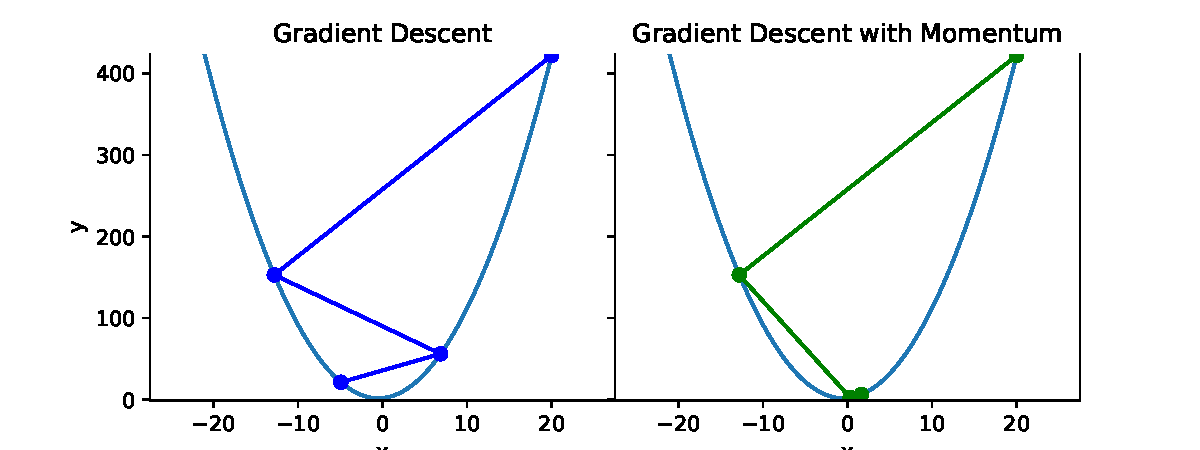
\includegraphics[width=1\textwidth]{report/figures/GD_momentum.pdf}
    \label{fig:gd-momentum}
\end{center}
Fig.\ref{fig:gd-momentum} illustrates how conventional gradient descent converges towards the minimum of the depicted quadratic function. On the right, one can observe gradient descent enhanced with momentum. Although the initial step is similar for both methods, the subsequent steps differ markedly. In the case of gradient descent alone, only the current gradient is considered as the slope. However, when employing gradient descent with momentum, the direction for the next step is determined by an accumulation of the current gradient and the previous gradients, resulting in a steeper descent as the first gradient slopes into negative direction of $x$.\par
In ADAM the learning rate is manipulated via the first moment estimate vector. The biased form is defined as 
\begin{equation}
    m_t=m_{t-1}\cdot \beta_1 + g_t\cdot (1-\beta_1)
    \label{eq:first-moment}
\end{equation}
The Eq.\ref{eq:first-moment} is called the biased mean of the gradient at iteration $t$, where $\beta_1$ has the default value of $0.9$. The unbiased mean gradient, defined as $\hat{m_t}$ is then multiplied with the adaptive learning rate and subtracted from $\theta_{t-1}$ to form the adapted set of parameters $\theta$. This inherits ADAM with the properties from Gradient Descent with Momentum as described.\par
It is important to notice that $m_t$ is initialized at $t=0$, being $m_0$, as a vector of zeros. This causes a bias towards $0$, which will be discussed in section \textit{Bias Correction}.

\subsection{Second Moment Vector}
The second moment vector is to implement an adaptive learning rate in ADAM, by adjusting the learning rate by considering the past gradients. This allows the model to take larger steps when far from the minimum and smaller steps when closer. This is possible, as the squared gradient is considered, meaning when the loss (error in a neural network) is large the learning rate is higher, and vice versa. Furthermore, by adjusting the learning rate this way, the initial learning rate is less relevant as it gets adjusted towards the data automatically. The methods idea was inspired by the Adadelta and RMSprop optimizer.\par
\begin{center}
    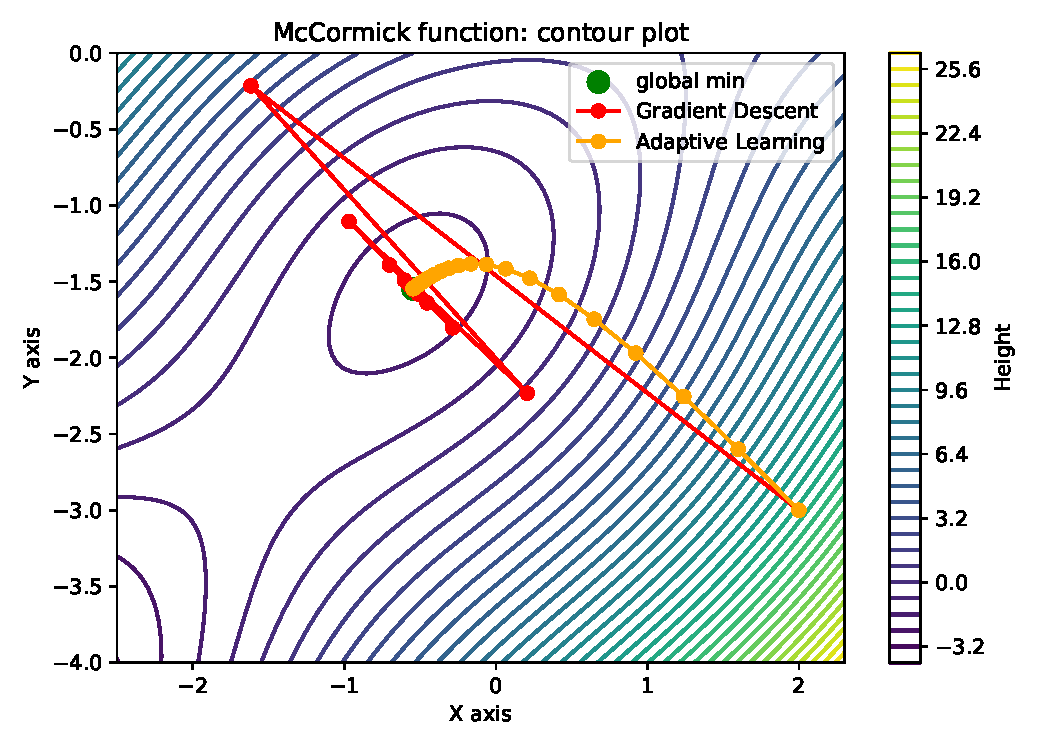
\includegraphics[width=0.8\textwidth]{report/figures/GD_rmsprop.pdf}
    \label{fig:gd-adapt-lr}
\end{center}\par
Fig.\ref{fig:gd-adapt-lr} shows a contour plot of the McCormick function, regularly explored for optimization due to its landscape. The graph illustrates the difference between classic GD compared to GD with the adaptive learning rate as implemented by ADAM. This is achieved by dividing the GD Learning rate by the root of the second moment vector. While classic GD is overshooting during the first couple of steps, GD with adaptive learning takes smaller steps, as the initial point is already close to the minimum, which adaptive learning knows due to its dependency on the gradient. This method is especially effective for high dimensional loss functions, where the initial steps of ADAM are usually larger than compared to GD, helping ADAM to potentially navigate the loss function to escape local minima.\par
In ADAM the learning rate is manipulated via the second moment vector. The biased form is defined as:
\begin{equation}
    v_t = v_{t-1} \cdot \beta_2 + g_t^2 \cdot (1-\beta_2)
    \label{eq:second-moment}
\end{equation}
Eq.\ref{eq:second-moment} is called the biased uncentered variance of the gradient at iteration $t$. Where $\beta_2$ has a default value of 0.999. The vector $v_t$ is initialized as $v_0$ being a vector of zero causing a bias, similar to $m_t$ that will also be explained in section \textit{Bias Correction}. The squared unbiased second-moment vector $\sqrt{\hat{v_t}}$ divides the default learning rate in ADAM to make it adaptive.
\subsection{Bias Correction}
Bias correction is an essential step to ensure the accuracy and efficiency of the moment vectors, especially during the initial iterations. As both vectors are initialized as vectors of zero, a significant bias towards zero is evident in the initial steps. This can lead to smaller-than-ideal step sizes at the start of optimization. If not corrected, this can slow down the convergence of the algorithm, as the optimizer takes conservatively small steps when the step sizes are unduly influenced by the initial bias.\par
Bias correction is performed for both the first and second-moment vector :
\begin{enumerate}
    \item \textbf{First Moment Bias Correction}\par
    \(m_t\) is corrected by dividing it by \((1 - \beta_1^t)\), where \(\beta_1\) is the exponential decay rate for the first moment estimates, and \(t\) is the iteration step. As \(t\) increases, \((1 - \beta_1^t)\) approaches 1, and the bias correction becomes less significant.
    \item \textbf{Second Moment Bias Correction}\par
    Similarly, the second-moment vector \(v_t\) is corrected by dividing it by \((1 - \beta_2^t)\), where \(\beta_2\) is the exponential decay rate for the second-moment estimates. This adjustment compensates for the underestimation of the second moment, ensuring that the scaled gradient is divided by a more accurate estimate of its variance, leading to more appropriate step sizes.
\end{enumerate}
\begin{center}
    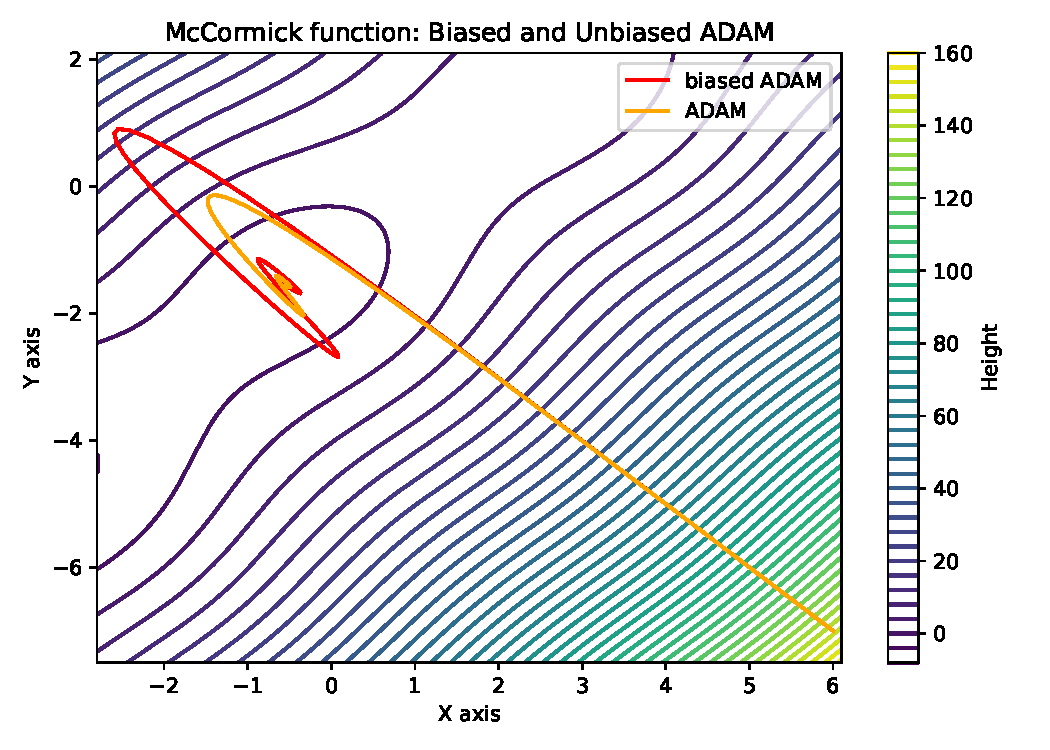
\includegraphics[width=0.8\textwidth]{report/figures/ADAM_bias.pdf}
    \label{Fig:adam_bias}
\end{center}
Fig.\ref{Fig:adam_bias} illustrates the impact of bias correction. Biased ADAM has a stronger tendency towards zero, which in this case leads to more significant overshooting, ultimately ending in slower convergence than unbiased ADAM.

\subsection{Summary Optimization Principles}
Fig.\ref{fig:adam_vs_gs} visually demonstrates the before-explained principles. The first-moment vector's role is critical in moderating the rate of gradient change, preventing erratic shifts that could derail convergence. Concurrently, the second-moment vector delicately adjusts the learning rate, ensuring it remains optimal as the algorithm approaches the minimum. This orchestrated interplay results in a smoother and more efficient path to convergence compared to traditional gradient descent methods, showcasing ADAM's optimization capability.
\begin{center}
    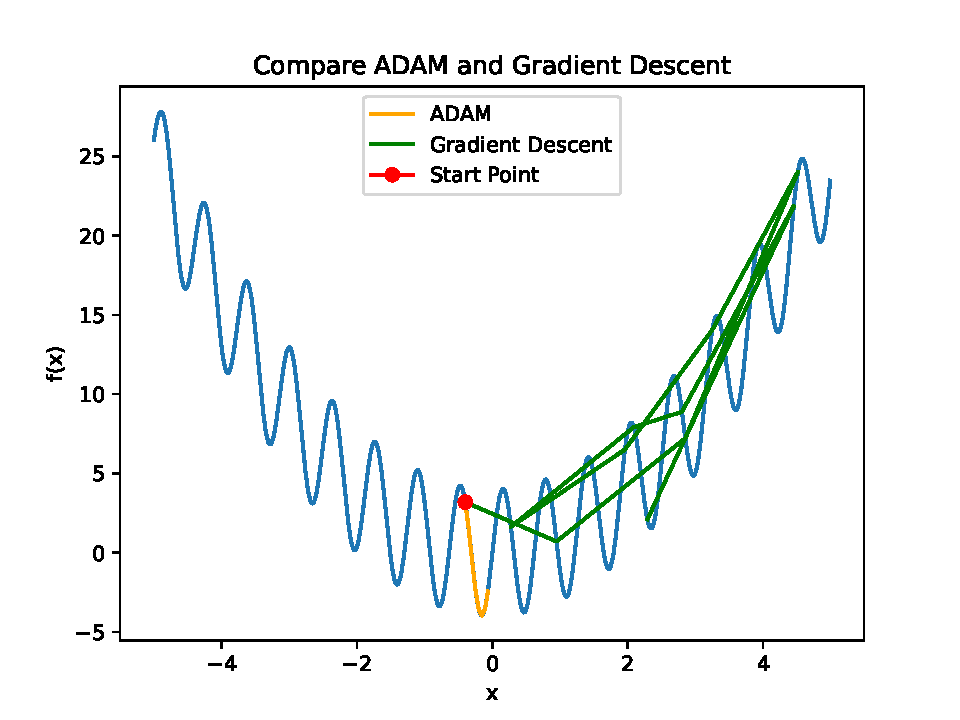
\includegraphics[width=0.8\textwidth]{report/figures/adam_vs_gradientdescent.pdf}
    \label{fig:adam_vs_gs}
\end{center}


\subsection{ADAM}
Definitions as in the forgoing section.
\subsubsection{Hyperparameters}
First, the hyperparameters need to be initialized:\\
$\alpha$ \par 
stepsize or the initial learning rate, usually around $0.001$ is picked. As mentioned the learning rate is manipulated by the second moment vector, meaning that small changes in the value assigned for $\alpha$ have little impact on the Opimitizer's performance. In genera, a higher learning rate can lead to faster convergence but risks overshooting the minimum, potentially causing instability. A lower learning rate ensures more stable convergence but may slow down the optimization process, possibly leading to getting stuck in local minima.\\
$\beta_1$\par 
is the exponential decay rate for the first moment vector, usually around $0.9$. A higher \(\beta_1\) value (close to 1) gives more weight to past gradients, potentially smoothing out the optimization but risking a slower reaction to recent changes. A lower \(\beta_1\) decreases memory, making it more responsive to new gradients but possibly more volatile.\\
$\beta_2$\par
is the exponential decay rate for the second moment vector, usually around $0.999$. A higher \(\beta_2\) value increases the influence of past squared gradients, leading to more stable but smaller learning rates and therefore slower updates, as it might not react quickly to changes in gradient variance. A lower \(\beta_2\) makes the algorithm more sensitive to recent changes in gradient variance, which can accelerate learning but increase the risk of instability.\\
$\epsilon$ \par
is for computational purposes to avoid division by zero. Can be picked according to computational capabilities between $10^{-5}$ and $10^{-8}$.

\subsubsection{Model Dependent Parameters}
After the hyperparameters, the model dependenent parameters are set:\par
$f(\theta)$ being the Stochastic loss function with parameters $\theta$. In the context of training neural networks, the stochastic objective function refers to the loss or cost function evaluated on a randomly selected subset (mini-batch) of the training data.\par
$t=1$ the initial step in the algorithm\par
$\theta_0$ initial parameters\par
$m_0=0$ first moment vector initializes as a vector of zeros\par
$v_0=0$ second moment vector initializes as a vector of zeros

\subsubsection{Algorithm steps}
Calculate step by step:
\begin{enumerate}
    \item \textbf{Gradient} \par
    \(g_t\) with respect to the parameters \(\theta\) at time step \(t\).
    \begin{equation}
        g_t= \nabla_{\theta} f_t(\theta_{t-1})
    \end{equation}
    \item \textbf{Biased first-moment estimate}
    \begin{equation}
        m_t = \beta_1 \cdot m_{t-1} + (1 - \beta_1) \cdot g_t
    \end{equation}
    
    \item \textbf{Biased second-moment estimate}
    \begin{equation}
        v_t = \beta_2 \cdot v_{t-1} + (1 - \beta_2) \cdot g_t^2
    \end{equation}
    
    \item \textbf{Bias correction of first-moment estimate}
    \begin{equation}
        \hat{m}_t = \frac{m_t}{1 - \beta_1^t}
    \end{equation}
    
    \item \textbf{Bias correction of second-moment estimate}
    \begin{equation}
        \hat{v}_t = \frac{v_t}{1 - \beta_2^t}
    \end{equation}
    
    \item  \textbf{Corrected parameters}
    \begin{equation}
        \theta_{t+1} = \theta_t - \alpha \cdot \frac{\hat{m}_t}{\sqrt{\hat{v}_t} + \epsilon}
    \end{equation}
    
    \item \textbf{Increase $t$} 
    \begin{equation}
        t = t + 1
    \end{equation}
    \item \textbf{Check parameter convergence}\par
    If $\theta_t$ converged, return $\theta_t$\par
    Else, rerun the steps one to eight
\end{enumerate}

\section{Performance Comparison}

This section evaluates the performance of the ADAM optimizer against other algorithms like SGD, ADAgrad, and RMSprop using the MNIST-Fashion dataset. This dataset, provided by Zalando, consists of 70,000 grayscale images across 10 fashion categories, used to test optimization algorithms in a more complex scenario than the traditional MNIST dataset of handwritten digits. The focus is on comparing how each optimizer performs in terms of minimizing loss and maximizing accuracy, using a model that normalizes pixel values and classifies images into categories. This practical comparison aims to identify which optimizer works best for this type of classification task, providing straightforward insights into their effectiveness.
\subsection{The MNIST-fashion Test Set}
One of the main benefits of the ADAM algorithm is its ability to optimize loss functions in more complex environments, such as neural networks. To investigate ADAMs efficiency compared to other algorithm, a classification task has been executed using different optimizers. These were ADAM, SGD, ADAgrad and RMSprop. The classifcation task at hand is the \textit{MNIST-Fashion} problem.\par

The MNIST fashion dataset is a data set made by Zalando containing $70 000 \ ,28 \times 28$ images depicting 10 different classes of fashion items. Example can be seen in \textbf{Figure X} These $70 000$ images are then divided into a training set of $60000$ and a test set of $10000$
Each pixel stores the information of how dark it is ranging 0-255. Overall it is similar to the orginal MNIST dataset, which contains instead contain numbers and which pictures are structured in the same manner, but it is considered a harder classifcation task than the regular MNIST problem, which one  github blog shows can be accurately predicted with just one \hyperlink{https://gist.github.com/dgrtwo/aaef94ecc6a60cd50322c0054cc04478}{pixel}. 

\begin{figure}[h!]
    \centering
    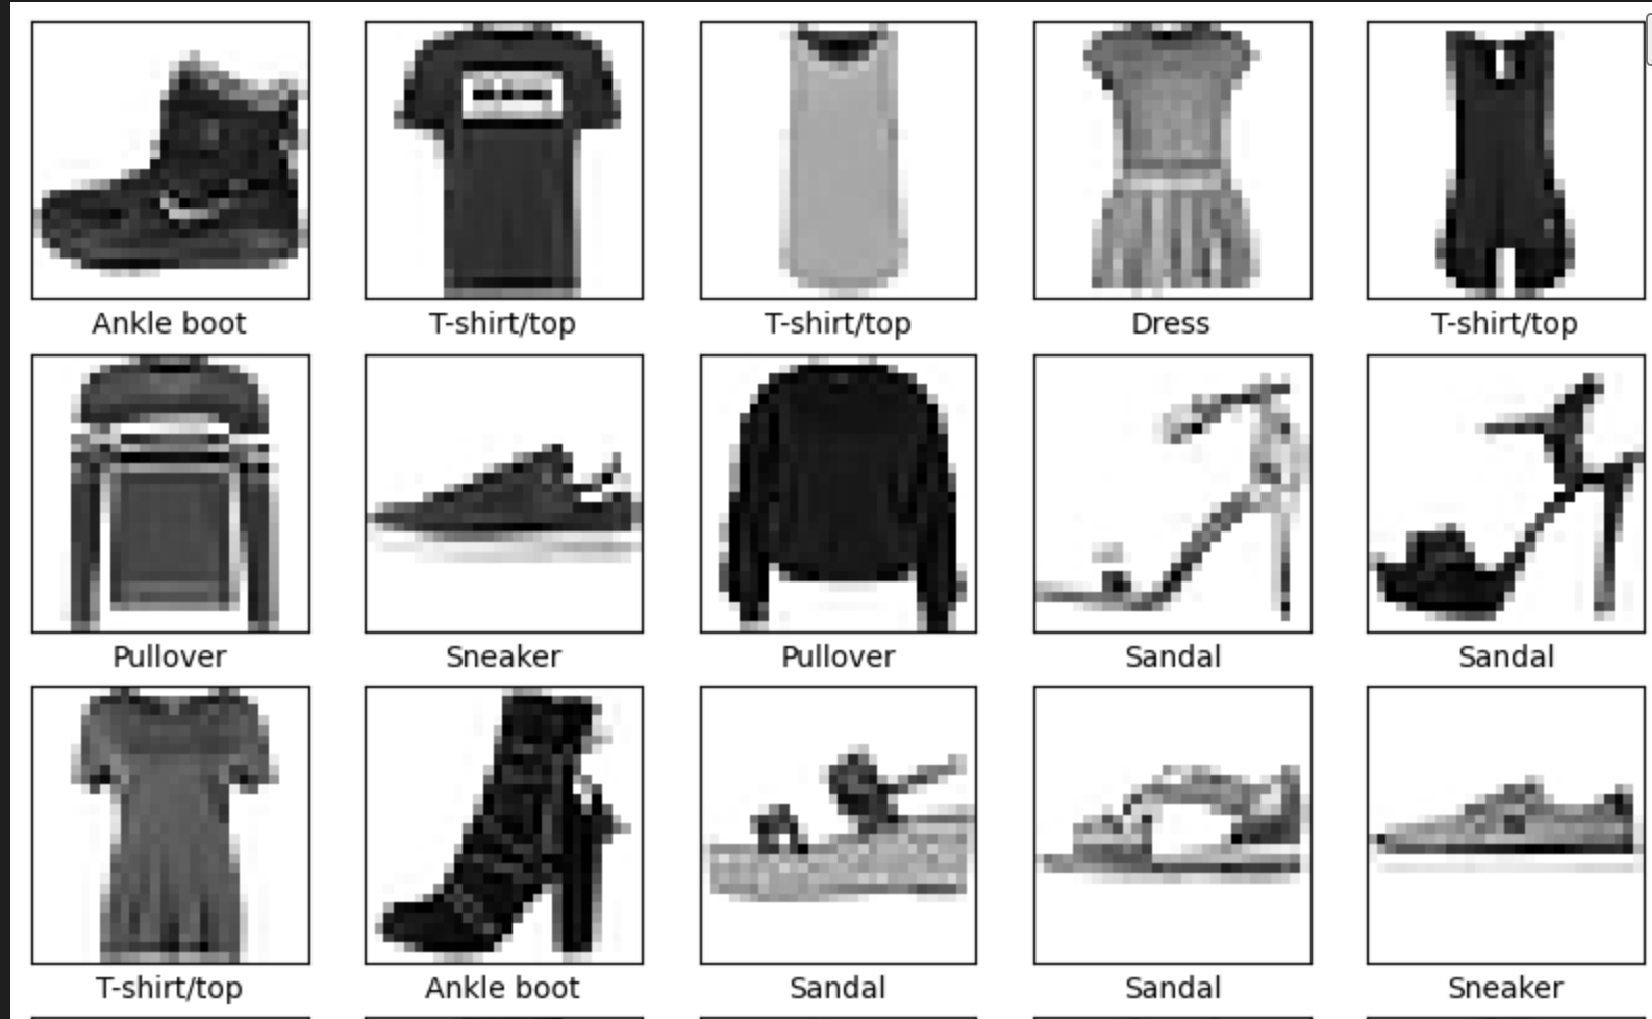
\includegraphics[width=0.42\linewidth]{report/figures/example_items.pdf}
    \caption{Enter Caption}
    \label{fig:enter-label}
\end{figure}

\subsection{Model Build}
To normalize the values, each pixels grey scale attribute was divided by 255, to make it range from 0-1 instead of 0-255, this is to make training easier due to smaller range.\par
Each model has 128 neurons and uses ReLu as an activation function in the first layer. Since we are looking to classify the the images into 10 different categories, there is 10 neurons in the second layer, using the softmax function to get the probabilities of each item of clothing. \par
The models are trained using the SpareCategoricalEntropy loss function, which multiplies the predicted probability and the actual probability to calculate the loss. This means that there is a vector containing the actual class (it being represented as 1 for the class and 0 for the other) and then a vector containing the probability assigned by the model of the image being each of the classes. By logging it it would mean that if you have a perfect match, where the entire probability is put on the actual class, it would be equal to 0. You want to \textit{minimize} the function. 


\subsection{Entropy Minimization and Training Set Accuracy}
In Figure \ref{fig:ATE}, each of the four optimization functions has been run to minimize the entropy loss function and tested on how accurate they are on the test set; both were compared to the number of epochs executed. This test yields a clear result: the ADAM optimizer is faster to converge to a minimum value for the entropy loss, as well as reaching the highest accuracy on the training set. Both SGD and RMSprop eventually converge towards the same minimum value as ADAM around the $\approx 350$ epoch for the entropy and the same maximum accuracy. However, Adagrad is outperformed in both entropy minimization and accuracy maximization by the other optimizers.
\begin{center}
    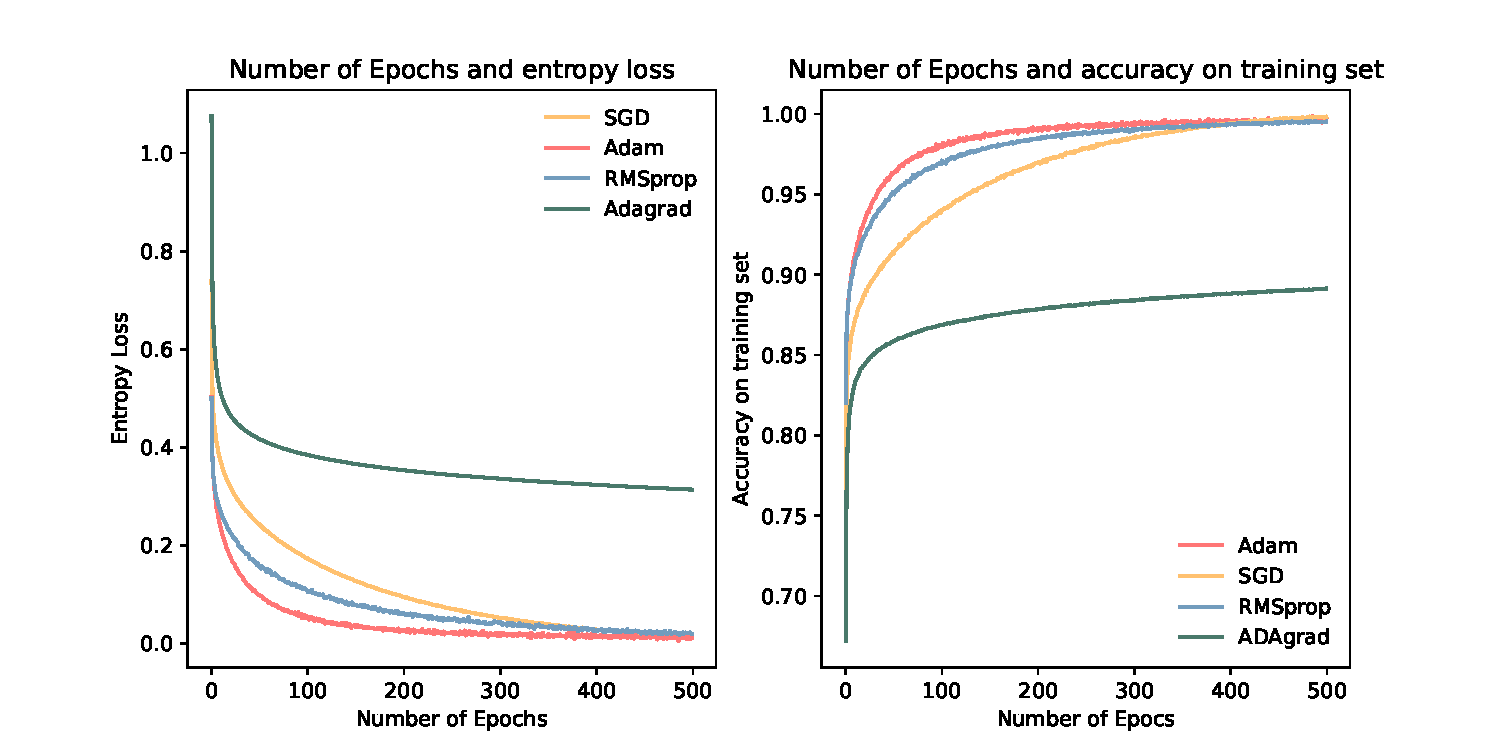
\includegraphics[width=1\textwidth]{report/figures/accuracy_training_and_entropy.pdf}
    \label{fig:ATE}\\
\end{center}
\subsection{Test Set Accuracy and Time Consumption}
In  Figure \ref{fig:TA} each of the four optimizing have been plotted on performance on the test set compared to the number of epochs and have also been compared in terms of time consumption to train the models with a given amount of epochs. \par
Adam is again the optimizer which yields the quickest convergence to a maximum accuracy on the test set. Followed suit by the RMSprop optimizer and SGD being close as well, Adagrad does again seem to not be able to reach the same accuracy as the other optimizers. Adam,SGD and RMSprop all yield noisy data in terms of prediction around the 0.89 threshold, which seems to be a kind of maximum accuracy that can be achieved with the specific parameters the models were trained on. Further, it seems as if SGD is the strongest performer in overall accuracy at around this point. ADAgrad does not deliver as noisy of a prediction but instead converges towards an overall lower accuracy than the other models. \par

In terms of time, all optimizers seem to train the models in linear time, with SGD being the fastest and Adam being the slowest.

\begin{center}
    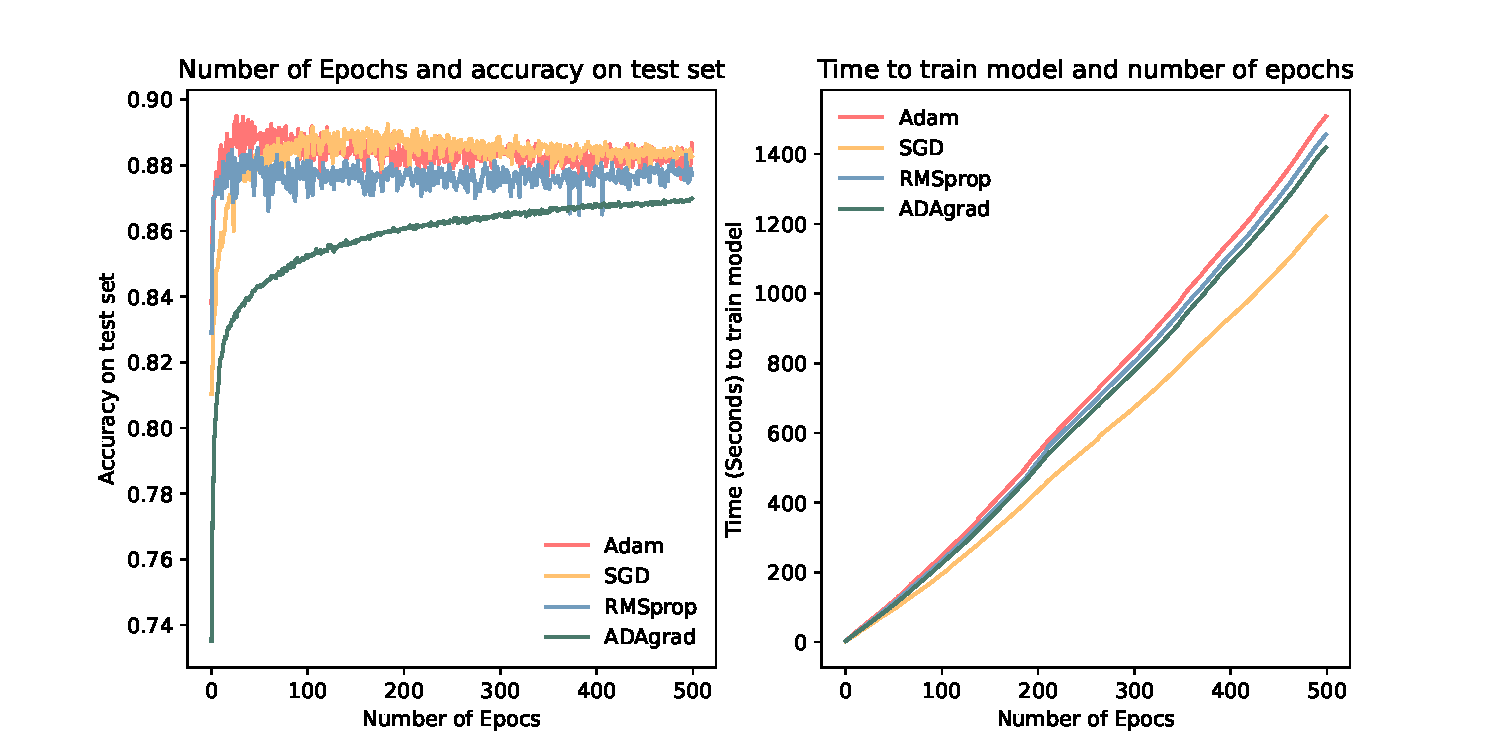
\includegraphics[width=1\textwidth]{report/figures/time_and_accuracy.pdf}
    \label{fig:TA}\\
\end{center}




\subsection{Results Discussion}

 From the results section, we can gather that ADAM, as outlined in the Method section does indeed provide a fast minimization of the loss function compared to the other optimizers, furthermore, it converges quicker to a higher accuracy when looking at results from both test and train sets. This was achieved in a similar time frame as other optimizers albeit slightly slower, especially for a higher number of epochs. \par
 Therein lies Adam's greatest benefit, the fast minimization. However, the result also shows that although SGD takes more epochs to converge towards its result, it eventually reaches the same accuracy and minimization of the loss function as ADAM. SGD also performs this slightly faster than ADAM in terms of time. SGD also reaches a more consistent higher accuracy on the test set around the 100 epoch mark. It is important to note that this occurs when the accuracy becomes noisy on the graph, probably due to overfitting for error, but this remains consistent with some reporting of SGD creating better-generalized models than ADAM in some cases (Gupta et al., 2021). \par
 To counteract this and increase performance there is the modification AdamW which adjusts the weights separately from the optimization steps, which can lead to better general models that simulate SGD.\par
 Another approach is to begin training a model with Adam for quick convergence and then switch to SGD for the latter training stages to increase performance on unseen data.

\section{Conclusion}

In conclusion, our investigation into the ADAM optimization algorithm highlights its ability to navigate the complex landscapes of loss functions within neural network architectures efficiently. By adeptly combining the mechanisms of RMSprop and Momentum within the stochastic gradient descent framework, ADAM exhibits remarkable proficiency in managing dynamic learning rates and leveraging momentum to expedite convergence. Our comparative analysis, particularly within the context of the MNIST-fashion classification task, further underscores ADAM's effectiveness. It outperforms traditional optimizers like SGD, ADAgrad, and RMSprop in minimizing entropy loss and enhancing test set accuracy, despite occasional preferences for the simpler, more generalizable SGD or the modified ADAMW in certain scenarios. This study affirms ADAM's robustness and adaptability across diverse machine-learning tasks.




% CODE FOR APPENDIX
\onecolumn
\newpage
\pagestyle{fancy}


\section{Appendix}
\subsection{Sources}
\begin{itemize}
    \item Gupta, A., Ramanath, R., Shi, J. \& Keerthi, S.S., 2021. Adam vs. SGD: Closing the generalization gap on image classification. In: Proceedings of the OPT2021: 13th Annual Workshop on Optimization for Machine Learning. \href{chrome-extension://efaidnbmnnnibpcajpcglclefindmkaj/https://opt-ml.org/papers/2021/paper53.pdf}{24-03-2024}
\end{itemize}

\subsection{Source Code}
All Notebooks and Visualizations including detailed code can be found in our GitHub-Repository:\par
\href{https://github.com/jakthehut/ADAM-Optimizer}{https://github.com/jakthehut/ADAM-Optimizer}


\end{document}